\section{Approach}

\begin{figure*}[t!]
\begin{center}
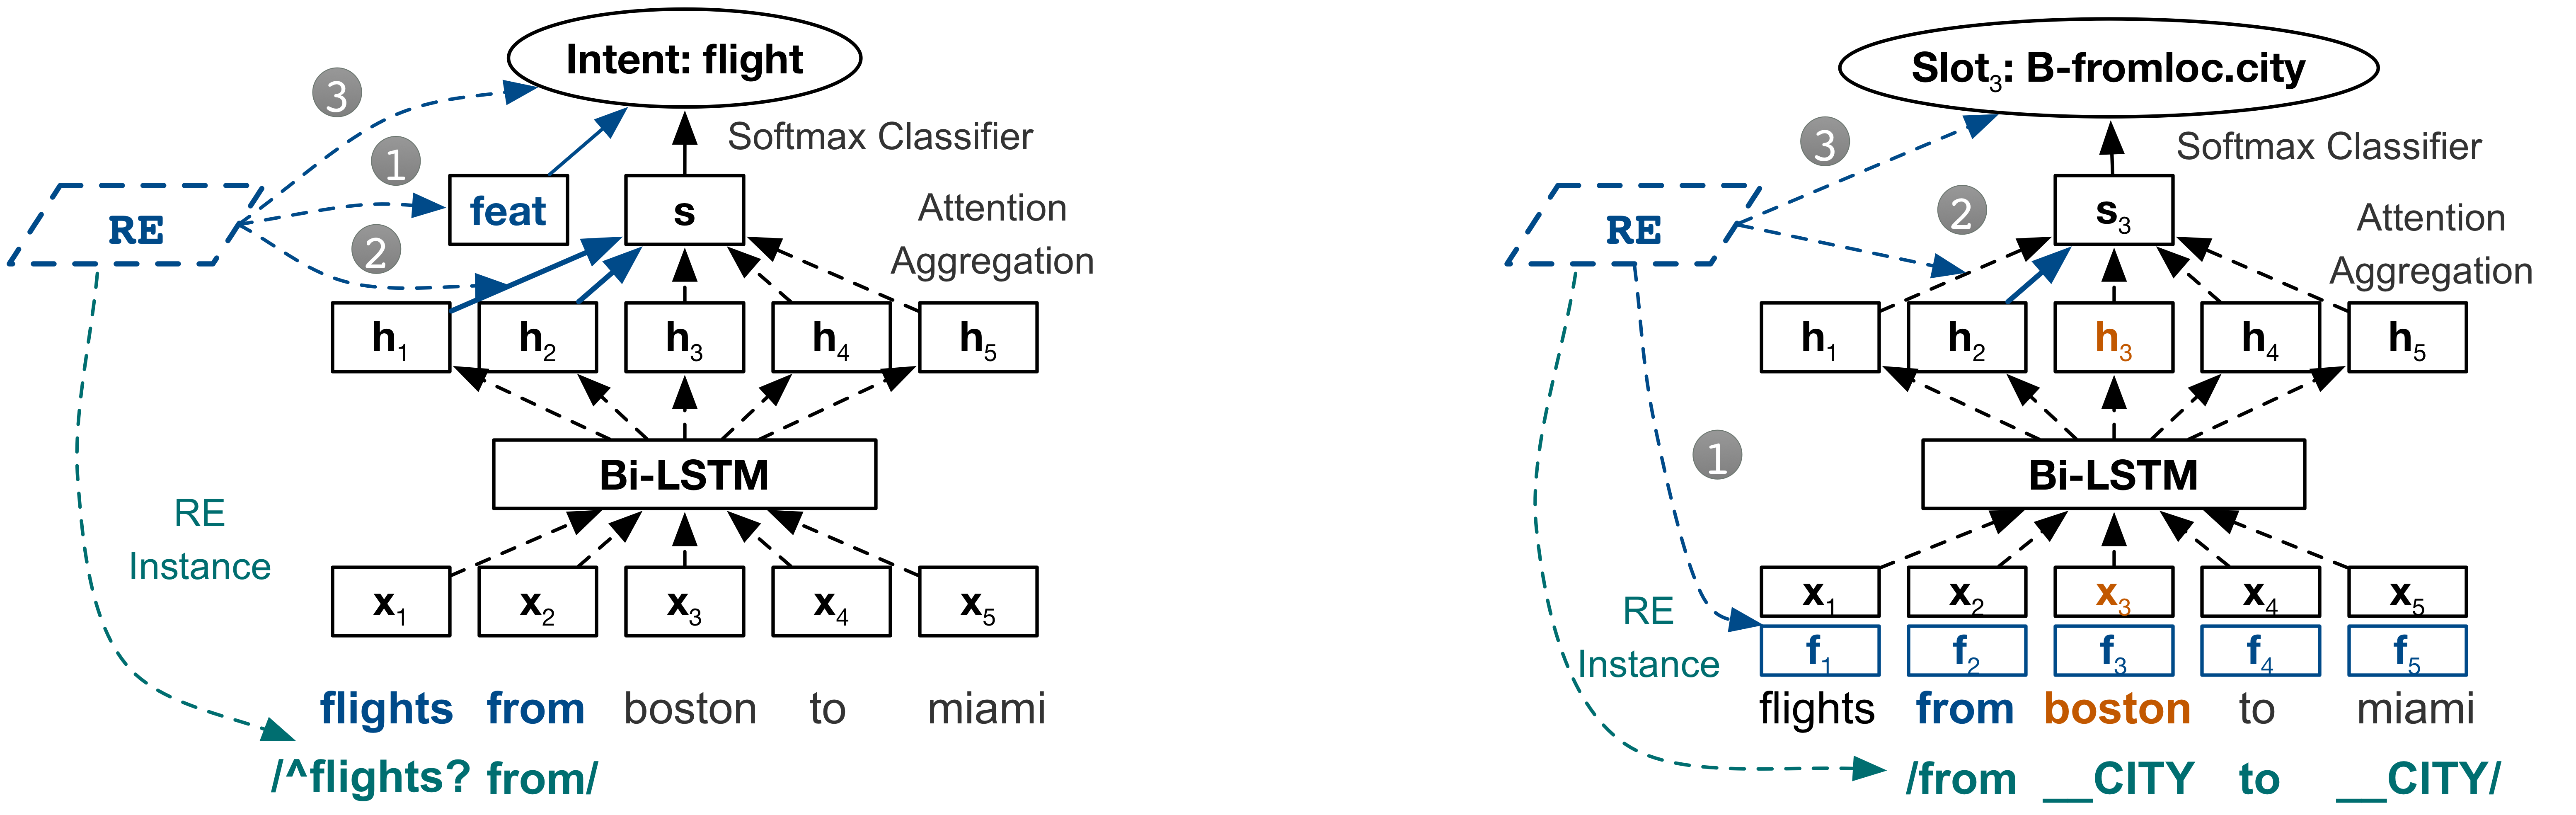
\includegraphics[width=0.85\textwidth]{figure/re_nn_overview.png}    
\caption{Overview of our methods. The left side shows the methods for intent detection, and the right side shows an example for predicting the slot lable for the word \textsl{\underline{boston}}. \circled{1}, \circled{2}, \circled{3} refers to the methods in Sec.~\ref{fusion_with_input}, \ref{interact_with_module}, \ref{fusion_with_output} respectively, and the \RE that applies to the input sentence is shown in the bottom.}
\label{fig_overview}
\end{center}
\vspace{-1em}
\end{figure*}

As shown in Fig.~\ref{fig_overview}, we will discuss three kinds of methods of combining \NN and \RE for both intent detection and slot filling.

\subsection{Base Models}
We use Bi-directional LSTM (\BLSTM) as our base \NN model for both intent classification and slot filling, which proves to perform well in both of these two tasks \cite{liu2016attention}. 
% Further, to obtain sentence embedding for intent detection, we use a self-attention layer upon the \BLSTM output.
\paragraph{Intent Detection}
As shown in Fig.~\ref{fig_overview}, given the word embeddings $[\textbf{x}_1, ..., \textbf{x}_n]$ as input, where $n$ is the sentence length, \BLSTM outputs a vector $\textbf{h}_i$ for each word $i$. 
Then, we use a self-attention layer to compute the sentence embedding $\textbf{s}$:
\begin{equation}
\textbf{s} = \sum_{i}{\alpha_i\textbf{h}_i}, \quad \alpha_i=\frac{exp(\textbf{h}_i\textbf{Wc})}{\sum_{i}{exp(\textbf{h}_i\textbf{Wc})}}
\end{equation}
where  $\alpha_i$ is the attention for word $i$, $\textbf{c}$ is a randomly initialized context vector used to select informative words for classification, and $\textbf{W}$ is a weight matrix. 
Finally, $\textbf{s}$ is fed to a softmax classifier for intent classfication.

\paragraph{Slot Filling}
The model for slot filling is more straightforward. Given the output of \BLSTM, the tag prediction of the word $i$ is generated by a softmax classifier which takes $\textbf{h}_i$ as input.\footnote{The attention aggregation in Fig.~\ref{fig_overview} is only used for the method in Section \ref{interact_with_module}.}


\subsection{Fusion On the Input Side}
\label{fusion_with_input}
Similar to the stacking technique \cite{wolpert1992stacked}, a straightforward way to combine \RE and \NN is to use the output of \RE patterns as feature, and feed them as the input of \NN models.
\paragraph{Intent Detection}
Our \RE tag for intent detection is the same as the intent label.\footnote{If no \RE matches, we will assign a special tag indicating no matches. This process is applied to all the settings.} 
And due to the imperfection of the \RE, one sentence may have several \RE tags that are possibly conflict with each other.
For example, the sentence \textsl{\underline{list the delta airlines flights to miami}} may match a pattern \texttt{/list(\;the)?\;\_\_AIRLINE/} that output tag \emph{airline}, 
and another pattern \texttt{/list(\;\textbackslash w+)\{0,3\}?\;flights?/} that output tag \emph{flight} as well.
% \footnote{\texttt{\_\_WORD} matches a single word, which can be \texttt{/\textbackslash w+/}.}

% Many paper has proved that, embed the discrete feature is an effective method to combine features in \NN \cite{zeng2014relation, guo2017deepfm}. 
Since there may exist several \RE tags for each sentence, we average the tag embeddings to form an aggregated embedding as input. 
Then, there are two ways to add this embedding: (1) append it to the embedding of every input word, (2) append it to the input of the softmax classifier (see \circled{1} in the left part of Fig.~\ref{fig_overview}).
Note that, in the first method, the tag embedding is actually copied $n$ times, where $n$ is the sentence length. 
In our pilot experiments, we find that the copied tag embeddings tend to dominate the input in few-shot settings, which makes \NN heavily relies on \RE output, and therefore makes the fusion performance similar to the performance of \RE alone. Consequently, we adopt the second method in this paper.

\paragraph{Slot Filling}
Since the output of slot \RE patterns output word-level tags, as shown in \circled{1} in the right part of Fig.~\ref{fig_overview}, we can simply embed and average the \RE tags into a vector $\textbf{f}_i$ for each word, and append it to the corresponding word embedding $\textbf{w}_i$. 
Further, since our slot labels follow the BIO annotation paradigm, we also extend the slot \RE tags to the BIO format. For example, the \RE tag of phrase \textsl{\underline{new york}} is \emph{B-city I-city} if its original tag is \emph{city}.

\subsection{Fusion on the NN Module Side}
\label{interact_with_module}
Since the \RE pattern itself has already highlighted informative words for the output tag, it can therefore help us guide the attention module in \NN.
As shown in \circled{2} in Fig.~\ref{fig_overview}, the bold blue arrows and words indicates the informative words marked by \RE for this prediction.
\paragraph{Intent Detection}
Taking the sentence in Table \ref{atis_sample} for example, the pattern \texttt{/\textasciicircum flights?\:from/} that leads to tag \emph{flight} means that, \textsl{\underline{flights from}} are key words to decide the intent \emph{flight}. Therefore, the attention module in \NN should attend to these two words to make correct prediction. 

Different from the base intent model, we make two changes to better incorporate the guidance from \RE.
First, since each intent has its own informative words, using a single sentence embedding, which is produced by only one set of attention, would make the attention less focused. 
% Considering we also know the intent that each \RE points to, 
Therefore, we let each intent $i$ use diffenrent attentions $\textbf{a}_i$, which is then used to generate the sentence embedding $\textbf{s}_i$ for that intent specifically:
\begin{equation}
\textbf{s}_i = \sum_{j}{\alpha_{ij}\textbf{h}_j}, \quad
\alpha_{ij}=\frac{exp(\textbf{h}_j\textbf{W}_a\textbf{c}_i)}{\sum_{j}{exp(\textbf{h}_j\textbf{W}_a\textbf{c}_i)}}
\label{label_att_eq}
\end{equation}
where $\textbf{c}_i$ is the context vector for intent $i$ which is used to compute attention, $\textbf{h}_j$ is the \BLSTM output for word $j$, and $\textbf{W}_a$ is a weight matrix.

The probability $p_i$ that the input sentence expresses intent $i$ is computed by:
\begin{equation}
p_i = \frac{logit_i}{\sum_{i}{logit_i}}, \quad\quad logit_i=\textbf{w}_i\textbf{s}_i + b_i 
\label{label_prob_eq}
\end{equation}
where $\textbf{w}_i$, $logit_i$, $b_i$ are weight vector, logit, and bias for intent $i$ respectively.

Second, apart from indicating a sentence expressing intent $i$ (\textbf{\emph{positive patterns}}), an \RE pattern can also indicate that a sentence should not be labeled as intent $i$ (\textbf{\emph{negative patterns}}). Therefore, to make use of negative patterns, we use another set of attention to compute a new set of logits for each intent using Eq.~\ref{label_att_eq} and \ref{label_prob_eq}. By denoting the logits computed by positive patterns as $logit_{pi}$, and the ones computed by negative patterns as $logit_{ni}$, the final logit for intent $i$ is then: 
\begin{equation}
logit_i = logit_{pi} - logit_{ni}
\end{equation}

To use \RE patterns to guide the attention, we add an attention loss to the final loss:
\begin{equation}
loss_{att} = \sum_{i}{m_i\sum_{j}{t_{ij}log(\alpha_{ij})}}
\label{att_loss}
\end{equation}
where $t_{ij} = 0$ when none of the matched patterns that lead to intent $i$ mark word $j$ as informative (\textbf{\emph{clue word}}), otherwise $t_{ij} = 1/k_{i}$ where $k_i$ is the number of clue words mark by \RE for intent $i$. $m_i$ is a 0-1 indicator that equals 1 only when there is a matched \RE that leads to intent $i$. We use Eq.~\ref{att_loss} to compute positive attention loss $loss_{att\_p}$ for positive patterns and negative attention loss $loss_{att\_n}$ for negative ones. The final loss is:
\begin{equation}
loss = loss_{c} + \beta_p loss_{att\_p} + \beta_n loss_{att\_n}
\end{equation} 
where $loss_{c}$ is the original classification loss, $\beta_p$ and $\beta_n$ are weights for the two attention losses.

In practice, while with some noise, a positive pattern for intent $i$ can often be negative patterns for other intents. For example, the pattern \texttt{/\textasciicircum flights?\:from/} that leads to tag \emph{flight} also indicates that the sentence should not be labeled as tags like \emph{meal}, \emph{quantity}, and etc.
Therefore, we use the positive pattern for intent $i$ as the negative patterns for other intents in our experiments.

\paragraph{Slot Filling}
While we can apply the same \textbf{\emph{two-side attention}} (positive and negative attention) method as we do in intent prediction, we face an efficiency problem in slot filling. Since we need to assign a label for each word, if we still compute attention for each tag, we will have to compute $2\times L \times n^2$ attention values for one sentence, where $L$ is the number of tags and $n$ is the sentence length. Considering the BIO tagging format further doubles the number of tags, this will result in a lot of computation and memory storage. 

Therefore, we use the simplified version of the two-side attention. Specifically, all the tags share the same set of positive and negative attention, and therefore we have only one sentence embedding $\textbf{s}_{pi}$ generated from positive attention, and another embedding $\textbf{s}_{ni}$ from negative attention for each word $i$. The final prediction $\textbf{p}_i$ for word $i$ is then:
\begin{equation}
\begin{split}
\textbf{p}_i = softmax((\textbf{W}_p [\textbf{s}_{pi}; \textbf{h}_i] + \textbf{b}_p) \\- (\textbf{W}_n [\textbf{s}_{ni}; \textbf{h}_i] + \textbf{b}_n))
\end{split} 
\end{equation} 
where $\textbf{W}_{p}$, $\textbf{W}_{n}$, $\textbf{b}_{p}$, $\textbf{b}_{n}$ are weight matrices and bias vecotrs for positive and negative attention respectively. Here we append the \BLSTM output $\textbf{h}_i$ to $\textbf{s}_{pi}$ and $\textbf{s}_{ni}$ because the word $i$ itself also plays an important part in identifying its slot label.

\subsection{Fusion on the Output Side}
\label{fusion_with_output}
The final type of combination is to use \RE to modify the output of \NN, and the method is the same for the two tasks (see \circled{3} in Fig.~\ref{fig_overview}). 

% Therefore, instead using a teach-student framework, this enables us to directly influence the logits of each label in a trainable way, so that we do not need to assign a weight for each pattern, and significantly reduces the number of hyper-parameters.

As mentioned in Section \ref{re_desc}, the slot \RE patterns used in this section only output a simplified version of the slot label.
Since the \RE tag is related to the slot label, we can further annotate which slot labels that each \RE will lead to.
% To make connections between the \RE tag and the slot label, we further annotate all the slot labels that the output tag may lead to.
For example, a pattern that outputs tag \emph{city} will lead to three slot labels: \emph{fromloc.city}, \emph{toloc.city}, \emph{stoploc.city}.
% Actually, annotating this kind of connections is not difficult, since the \RE tags are generally somewhat related to the target label that we are trying to predict, otherwise the \RE tags will not be able to provide useful information for the prediction.

Let $z_i$ be a 0-1 indicator of whether at least one \RE pattern that leads to target label $i$ matches the input sentence, then the final logits of label $i$ for the sentence (or a specific word for slot filling) is: 
\begin{equation}
logit_i = logit'_i + w_i z_i
\end{equation}
where $logit'_i$ is the logit produced by the original \NN, and $w_i$ is a trainable weight indicating the overall confidence for patterns that lead to label $i$.
Here we do not assign a trainable weight for each pattern because there is a good chance that there are only limited sentences matching a specific \RE.

We modify logit instead of the final probability because logit is a real value, which matches $w_i z_i$ better than probability. Further, kagglers have also proved emperically that, ensembling with logits is often better than ensembling with the final probability (see the ensemble version of Juan et al.~\shortcite{juan2016field}), which is also the reason that we operate on logit instead of probability in Sec.~\ref{interact_with_module}.
% Further, if we have strong prior confidence on the patterns, we can also easily incorporate these human-assigned pattern weights by simply multiplying it to $w_i$.


